\documentclass{ctexart}

\usepackage{graphicx}
\usepackage[defaultmono,scale=0.85]{droidsansmono}
\usepackage[hmargin=1.1in,vmargin=1in]{geometry}

\newcommand{\theauthor}{Sparky\_14145}

\input{personal_info/info.tex}

\title{计算机图形 作业四}
\author{\theauthor}

\begin{document}
    \maketitle

    \section{函数流程}

    \subsection{recursive\_bezier}

    (其实并不 recursive 的一个算法)

    根据已有的点 $P_1, P_2$ 计算下一个点 $P'_1$ 的公式为:

    \[
        P'_1 = t \times P_2 + (1-t) \times P_1
    \]

    根据公式,先创建两个 \verb|std::vector<Point2f>|,一个用来存已知的点,另一个用来存
    迭代计算出来的点,每次将要求出的点全部算出来后用它们覆盖已知的点。最后在只剩下 1 个点的
    时候将这一个点返回就行了。

    \subsection{bezier}

    设定一个 $\Delta t$,然后将 $t$ 从 0 开始每次加上 $\Delta t$,直至 $t = 1$,并
    以此调用上面提到的 \texttt{recursive\_} \texttt{bezier},再将返回的点画出来就可以了。

    \section{运行结果}

    我将 \verb|bezier| 函数绘制的点设为绿色,而内置的参考结果是红色,则两者重合的部分为
    黄色。

    从图中(\texttt{my\_bezier\_curve.png})可以看到两者的的匹配较好,由此证明实现正确。

    \begin{center}
        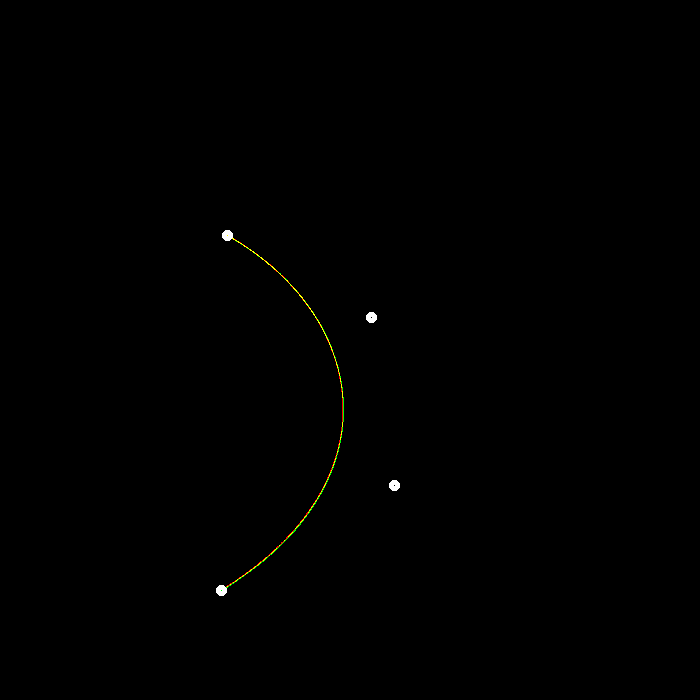
\includegraphics[width=0.3\textwidth]{pics/result.png}
    \end{center}
\end{document}